\documentclass[11pt]{amsart}


\usepackage{geometry}                % See geometry.pdf to learn the layout options. There are lots.
\geometry{a4paper}                   % ... or a4paper or a5paper or ...
%\geometry{landscape}                % Activate for for rotated page geometry
\usepackage[parfill]{parskip}    % Activate to begin paragraphs with an empty line rather than an indent
\usepackage{enumitem}
\usepackage{graphicx}
\usepackage{amssymb}
\usepackage{amsmath}
\usepackage{cancel}
\usepackage{epstopdf}
\DeclareGraphicsRule{.tif}{png}{.png}{`convert #1 `dirname #1`/`basename #1 .tif`.png}
\usepackage{breqn}
\usepackage{float}

\title{Econ 210C Problem Set \# 3}
\author{Minki Kim}
%\date{}                                           % Activate to display a given date or no date

\begin{document}




\maketitle

\section{Variable labor supply in the RBC model}
\begin{figure}[H]
	\centering
	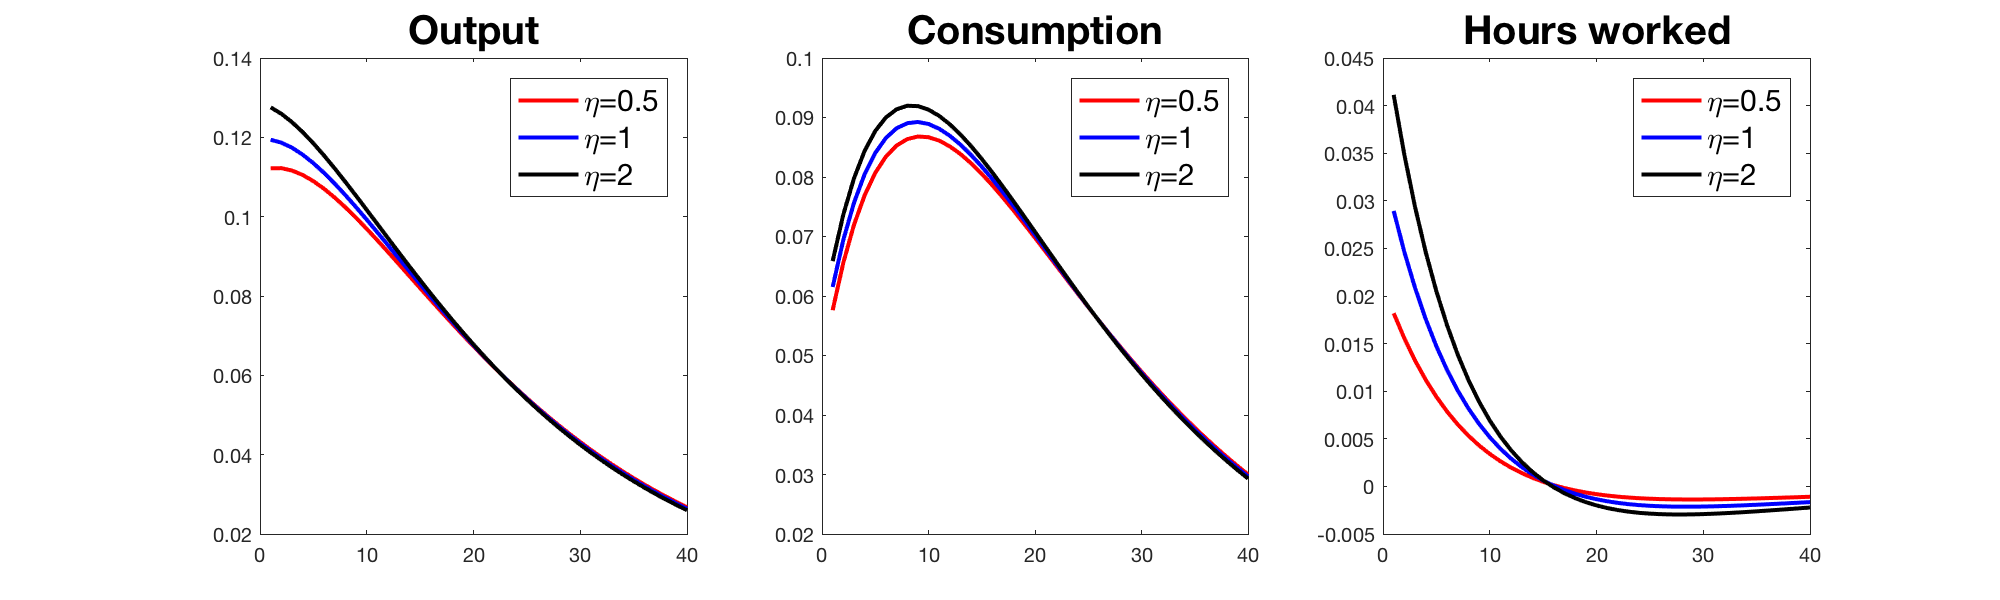
\includegraphics[width=\textwidth]{Q1}
	\caption{Impulse responses with varying $\eta$}
\end{figure}

\begin{table}[H]
	\centering
	\begin{tabular}{ccccc}
		\hline \hline 
		& $\eta=0.5$  & $\eta = 1$          & $\eta = 2$ & Data  \\
		\hline 
		$Stdev(Y)$ &  1.54    & 1.64    & 1.74    & 1.72     \\
		$Stdev(C)$ &  0.97    & 1.02   & 1.08       & 1.27 \\
		$Stdev(L)$ &   0.23   &  0.37   & 0.53     &  1.59 \\
		\hline
	\end{tabular}
	\caption{Response to a transitory discount factor shock}
\end{table}
As one would expect, the fits get better as we calibrate the Frisch elasticity to bigger values. A large Frisch elasticity generates stronger intertemporal substitution of labor suppply, and hence amplifies the effect of shocks. However, even with a large Frisch elasticity, consumption is too smooth, and the volatility of hours generated from the model falls short of the empirical counterpart. 

\section{Variable capital utilization in an RBC model}
\begin{enumerate}[label=(\alph*)]
	\item The Lagrangian of the firm's profit maximization problem is: 
	\begin{align*}
	\mathcal{L} =& \mathbb{E}_t \sum_{s} \left( \prod_{k=1}^{s} \left(1 + R_{t+k} \right) \right)^{-1} \\\
	 &\times \left[  \left( U_{t+s} K_{t+s-1}  \right)^{\alpha} \left(Z_{t+s} N_{t+s}  \right)^{1-\alpha}  - W_{t+s} N_{t+s} - I_{t+s} + q_{t+s} \left( -K_{t+s} + (1-\delta(U_t))K_{t+s-1} + I_{t+s} \right) \right] 
	\end{align*}
	The first order conditions are: 
	
	\begin{align*}
	\frac{\partial \mathcal{L}}{\partial N_{t}} : \quad & W_{t} = (1-\alpha)  \left( U_{t} K_{t-1}  \right)^{\alpha} \left(Z_{t} N_{t}  \right)^{-\alpha} \\
	\frac{\partial \mathcal{L}}{\partial I_{t}} : \quad & q_t = 1 \\
	\frac{\partial \mathcal{L}}{\partial K_{t}} : \quad & q_t = \mathbb{E}_t \frac{1}{1 + R_{t+1}} \left[ \alpha \left( U_{t+1} K_{t}  \right)^{\alpha} \left(Z_{t+1} N_{t+1}  \right)^{1-\alpha}  + q_{t+1} \left( 1-\delta(U_{t+1}) \right) \right] \\
		\frac{\partial \mathcal{L}}{\partial U_{t}} : \quad & q_t \delta^{'}(U_t) K_{t-1}  = \alpha \left( U_t K_{t-1} \right)^{\alpha -1} K_{t-1} \left( Z_t N_t \right)^{1-\alpha} 
	\end{align*}
	
	Combining the second and the third equations, we get the expression for the rental rate of capital. 
	\begin{equation*}
	R_{t+1} = \alpha \left( U_{t+1} K_{t}  \right)^{\alpha} \left(Z_{t+1} N_{t+1}  \right)^{1-\alpha} - \delta(U_{t+1})
	\end{equation*}
	The rental rate depends on $U_t$ because both $MPK$ and depreciation rates depend on $U_t$. 
	
	\item Log linearized version of $q_t \delta^{'}(U_t) K_{t-1}  = \alpha U_t^{\alpha -1} K_{t-1}^\alpha \left( Z_t N_t \right)^{1-\alpha}$ is
	\begin{align*}
	&\check{q_t}+ \frac{\delta^{''}(\bar{U}) \bar{U}}{\delta^{'}(\bar{U})} \check{U}_t + \check{K}_{t-1} = (\alpha -1) \check{U_t} + \alpha \check{K_{t-1}}  + (1-\alpha) \left(  \check{Z_t} + \check{N_t}\right) 
	\end{align*}
	Using $\check{q_t}=0$ and $\check{Y_t} = \alpha \left( \check{U_t} + \check{K_{t-1}} \right) + (1-\alpha) \left(  \check{Z_t} + \check{N_t}\right)$, we can express $\check{U_t}$ in terms of $\check{Y_t}, \check{K_t}$, and $\Delta$. 
	\begin{align*}
	\check{U_t} = \frac{1}{1 + \Delta} \left( \check{Y_t} - \check{K_{t-1}}\right)
	\end{align*}
	
	\item The production function in a log-linear form is: 
	\begin{align*}
	\check{Y_t} &= \alpha \left( \check{U_t} + \check{K_{t-1}} \right) + (1-\alpha) \left(  \check{Z_t} + \check{N_t}\right) \\
	& = \frac{\alpha}{1 + \Delta} \left( \check{Y_t} - \check{K_{t-1}} \right) + \alpha \check{K_{t-1}} + (1-\alpha ) \left(  \check{Z_t} + \check{N_t}\right)
	\end{align*} 
	Isolate $\check{Y_t}$:
	\begin{align*}
	\check{Y_t} &= \frac{\Delta \alpha }{1 + \Delta - \alpha} \check{K_{t-1}} + \frac{(1+\Delta)(1-\alpha)}{1+ \Delta - \alpha} \left(  \check{Z_t} + \check{N_t} \right)  \\
	& = \check{Z_t} + \check{N_t} \quad \left( \text{when } \Delta = 0 \right) \\
	& = \alpha \check{K_{t-1}} + (1-\alpha) \left( \check{Z_t } + \check{N_t} \right)   \quad \left( \text{when } \Delta = \infty \right)
	\end{align*}
	\begin{enumerate}[label = (\roman*)]
    \item $\Delta = 0 $ means that the steady state capital utilization rate is zero. Hence no matter how big the capital stock is, it does not contribute to the output. Therefore, deviations of output from its steady state solely depend on technology and labor. 
    
    \item $\Delta = \infty$ means that steady state capital utilization rate is one. In this case, this model boils down to a model without capital utilization, since 100\% of capital stock is always used in production. Therefore, deviations of output from its steady state depend on all three inputs of the production function, with weights corresponding to the inputs same as the Cobb-Douglas coefficients. 
    
    \item Consider the case when $0 < \Delta < \infty$. In this case, the log linearized production function is written as: 
    \begin{equation*}
    \check{Y_t} = \frac{\Delta \alpha }{1 + \Delta - \alpha} \check{K_{t-1}} + (1-\alpha) \left( \check{Z_t} + \check{N_t} \right)+ \frac{\alpha (1-\alpha)}{1+ \Delta - \alpha} \left(  \check{Z_t} + \check{N_t} \right)
    \end{equation*}
    Since capital stock is not fully used in production, the contributions of $Z_t$ and $N_t$ in $Y_t$ is higher than when $\Delta = \infty$. 
    \end{enumerate}
    \item 
\end{enumerate}

\section{Homework in macroeconomics}
\begin{enumerate}[label = (\alph*)]
	\item The Lagrangian for the household's maximization problem is:
	\begin{equation*}
	\mathcal{L} = \left( C_m^\rho + C_h^\rho \right)^{\frac{1}{\rho}} - \left( \frac{1}{\eta} + 1 \right)^{-1} \left(  L_h + L_m \right)^{\frac{1}{\eta} + 1} + \lambda \left( W L_m - C_m \right) + \xi \left(L_h - C_h \right)
	\end{equation*}
	The first order conditions for the interior solutions are:
	\begin{align*}
	\left( C_m^\rho + C_h^\rho \right)^{\frac{1}{\rho} -1} C_m^{\rho-1} &= \lambda \\
	\left( C_m^\rho + C_h^\rho \right)^{\frac{1}{\rho} -1} C_h^{\rho-1} & = \xi \\
	\left(  L_h + L_m \right)^{\frac{1}{\eta} }  &=\lambda W \\
	\left(  L_h + L_m \right)^{\frac{1}{\eta} }  &= \xi 	 
	\end{align*}
	\item $\xi = \lambda W $
	\item $\xi = \lambda \left( \frac{C_m}{C_h} \right)^{1-\rho}$ \\
	\item Assuming an interior solution, $C_h = L_h = C_m W^{\frac{1}{\rho-1}}$
	\item 
\end{enumerate}

\section{$q$-Theory with Variable Capital Utilization}
\begin{enumerate}[label = (\alph*)]
	\item The Lagrangian of the firm's profit maximization problem is: 
	\begin{align*}
	\mathcal{L} =& \mathbb{E}_t \sum_{s} \left( \prod_{k=1}^{s} \left(1 + r_{t+k} \right) \right)^{-1} \\
	\begin{split}
	&\times \left\lgroup  Z_{t+s} \left( U_{t+s} K_{t+s-1}  \right)^{\alpha} L_{t+s}^{1-\alpha}  - W_{t+s} L_{t+s} - I_{t+s} \left[ 1 + \phi \left( \frac{I_{t+s}}{K_{t+s-1}} \right) \right] \right. \\
	& \qquad + q_{t+s} \left( -K_{t+s} + (1-\delta(U_t))K_{t+s-1} + I_{t+s} \right) \left. \right\rgroup
	\end{split}
	\end{align*}
	This problem is truly dynamic because the presence of an adjustment cost links the present and future period investment decisions. 
	\item 
\end{enumerate}
\section{Fiscal multiplier in the RBC model}

\end{document}
